\documentclass[11pt, a4paper]{article}

% Encoding
\usepackage[utf8]{inputenc}

% Hyphenation
\usepackage[english]{babel}

% Extended math environments
\usepackage{amsmath}
\numberwithin{equation}{section}

% Additional math fonts and symbols
\usepackage{amsfonts}
\usepackage{amssymb}

% Units and uncertainties
\usepackage{siunitx}
\sisetup{
    separate-uncertainty
}

% Margins
\usepackage[left=3.5cm, right=3.5cm, top=3cm, bottom=3cm, twoside]{geometry}

% Pictures
\usepackage{graphicx}

% Text color
\usepackage{color}

% Hyperlinks
\usepackage{hyperref}
\hypersetup{
    colorlinks = true,
    allcolors = {black}
}

% Better table layouts
\usepackage{booktabs}
\usepackage{multirow}
\usepackage{multicol}

% Page Header
\usepackage{fancyhdr}

% Float Barriers
\usepackage{placeins}

% Rotated figures
\usepackage{caption}
\usepackage{subcaption}
\usepackage{rotating}

% Wrapped figures
\usepackage{wrapfig}

\usepackage{float}

% Remarks
\newcommand{\remark}[1]{{\color{red}(#1)}}

% Code
\usepackage{listings}
\definecolor{dkgreen}{rgb}{0,0.6,0}
\definecolor{gray}{rgb}{0.5,0.5,0.5}
\definecolor{mauve}{rgb}{0.58,0,0.82}

\lstset{frame=tb,
	aboveskip=3mm,
	belowskip=3mm,
	showstringspaces=false,
	columns=flexible,
	basicstyle={\footnotesize\ttfamily},
	numbers=left,
	numbersep=4pt,
	numberstyle=\tiny\color{black},
	keywordstyle=\color{blue},
	commentstyle=\color{dkgreen},
	stringstyle=\color{mauve},
	breaklines=true,
	breakatwhitespace=true,
	tabsize=4,
	xleftmargin=1em,
	xrightmargin=0.8em
}

% Caption-Setup
\captionsetup{font={small}}
\renewcommand{\thefigure}{\thesection.\arabic{figure}}
\renewcommand{\thesubfigure}{\alph{subfigure}}
\renewcommand{\thetable}{\thesection.\arabic{table}}
\renewcommand{\thesubtable}{\alph{subtable}}

% Depth of TOC (Level: 1 sections, 2 subsections, 3 subsubsections)
\setcounter{tocdepth}{3}

% FANCYHDR SETUP
\pagestyle{fancy}
\fancyhead[EL,OR]{\thepage}
\fancyhead[ER]{\leftmark}
\fancyhead[OL]{\rightmark}

\renewcommand{\sectionmark}[1]{
\markboth{\thesection{} #1}{\thesection{} #1}
}
\renewcommand{\subsectionmark}[1]{
\markright{\thesubsection{} #1}
}

% Document Info
\title{Particles in a potential}

\author{Christopher Deutsch\footnote{christopher.deutsch@uni-bonn.de} \and Philip Hauer\footnote{philiphauer@googlemail.com}}

\date{\today}

\begin{document}

\begin{titlepage}

\maketitle

% ABSTRACT
\begin{abstract}
\noindent 
A set of two oppositely charged particles that interact via a two-particle potential in a finite volume in two dimensions is considered.
With a Random-Walk Metropolis algorithm one can simulate the time evolution of this system.
The focus of this report lies on the analysis of the temperature dependence in particular the average pair distance.
Additionally the behavior for different potentials and in three dimensions is also studied.
\end{abstract}

\end{titlepage}

% TABLE OF CONTENTS
\tableofcontents
% New page after TOC
\newpage

% CONTENT

\section{Introduction}
This report summarizes the results of the analysis of a two-dimensional system where only two kind of particles, a positive and a negative one are considered.
They interact via a potential which is given by
\begin{equation}
V_{ij} = \frac{q_i q_j}{\left| \vec{r}_i - \vec{r}_j \right|} + \frac{1}{\left| \vec{r}_i - \vec{r}_j \right|^8} \, \text{.} \label{Eq:Potential}
\end{equation}
For the analysis a Random-Walk Metropolis algorithm is used. It will be explained in chapter \ref{sec:Metropolis}.
The used algorithm depends on the temperature and this dependence is studied in chapter \ref{sec:Temperature}.
As an indicator for the phase of the system the average pair distance is monitored.
A visualization of the different phases was also done and can be found in the section \ref{sec:Visualisation}.
In addition to that some further researches with other potentials (e.g. Lennard-Jones potential) were done and the behaviour of this system in three dimensions was also analysed.
These further thoughts and results are explained in chapter \ref{sec:Further_Analysis}.


\section{Background}

\subsection{Canonical ensemble} \label{sec:Canonical_Ensemble}

The statistical ensemble describing a fixed number of particles~$N$ in a given volume~$V$, which is in thermal equilibrium with a heat bath of temperature~$T$, is the canonical ensemble.
Aim of this project is to sample states from a given ensemble with fixed $N, V, T$ and use these to calculate expectation values of certain observables.
For this the probability density for realizing a specific microstate of the ensemble needs to be known.
In statistical mechanics the probability density for a canonical ensemble to be in a microstate with energy eigenvalue~$E$ is given by \cite{schwabl}
\begin{align*}
	P = \frac{1}{Z} \exp\left[ -\beta E \right] \qquad \beta := \frac{1}{k_\mathrm{B} T}
\end{align*}
with the normalization factor $1/Z$, where $Z$ is the canonical partition function.
For a system of particles with an inter-particle potential~$V_{ij}$ and neglecting kinetic energies the canonical partition function
\begin{align*}
	Z = \int \prod_{i=1}^N \mathrm{d}\mathbf{r}_i \exp\left[ -\beta \sum_{i < j} V_{ij} \right]
\end{align*}
is a constant of the ensemble and the total energy of the system is
\begin{align*}
	E = \sum_{i < j} V_{ij} \, \text{.}
\end{align*}
Since the calculation of $Z$ is computationally expensive a sampling method without the need of a normalized probability density is desirable.
One such method is sampling using the Metropolis algorithm, which is introduced in the following section.


\subsection{Metropolis algorithm} \label{sec:Metropolis}
The Metropolis algorithm is a Markov-chain Monte-Carlo method for generating an autocorrelated sequence of random samples of a given probability distribution.
These samples can be used to approximate distributions for which direct sampling methods cannot be employed. \remark{Hier mehr?}
Hereafter a summary of the algorithm is given.\\

\noindent\textbf{Random-Walk Metropolis algorithm:}\\
For a given initial state~$x_0$ and target density~$P(x)$, a sequence of random samples~$\left( x_n \right)$ can be obtained using the following steps:
\begin{enumerate}
	\item \textbf{Trial change:}
		Propose a new state $y$ according to a symmetric proposal distribution $q(Y|x_n)$ depending on the current state $x_n$.
		
	\item \textbf{Accept-reject step:}
		Calculate the acceptance probability
		\begin{align}
			\alpha(x, y) = \min\left\{ \frac{P(y)}{P(x_n)}, 1\right\} \,\text{.}
			\label{eq:acceptance_probability}
		\end{align}
		Generate $u \sim \mathcal{U}(0, 1)$ and set the random sample~$x_{n+1}$ according to:
		\begin{align*}
			x_{n+1} = \begin{cases}
					y_n \,, & u \leq \alpha(x_n, y_n) \\
					x_n \,, & u > \alpha(x_n, y_n)
				\end{cases}
		\end{align*}
		
	\item \textbf{Repeat}
\end{enumerate}
Moreover the target density~$P(x)$ does not need to be normalized, since it only occurs as a fraction of densities in the accept-reject step.
Therefore this algorithm is suitable to sample from a canonical ensemble without the explicit calculation of the canonical partition function.


\section{Implementation}
For the simulations of the canonical ensemble the programming language \texttt{C++} was used.
In the following a summary of the core implementation details is given.

\subsection{Metropolis algorithm} \label{sec:Metropolis_alg}
Since the subject of this project requires the simulation of particles in two or three dimensions and different inter-particle potentials, a generic approach of implementing the algorithmic core was chosen.
The source code of the implementation is listed in appendix~\ref{sec:canonical_ensemble_source}.

The Metropolis algorithm is encapsulated in a class-template~\texttt{CanonicalEnsemble} taking a parameter \texttt{ParticleState} indicating the type used to describe the state of one particle.
For the case of two-dimensional charged particles this could be a \texttt{struct} containing three floating point members describing the particle charge~$q$ and two coordinates~$x, y$.
Each object of type \texttt{CanonicalEnsemble} has several important (inaccessible) members associated with it:
\begin{itemize}
	\item \texttt{state}:
		A dynamically allocated array of type \texttt{ParticleState} fully describing the state of the ensemble (i.e.\ the charges and coordinates of all particles).
		The current state can be queried using the \texttt{get\_state} member-function.
	
	\item \texttt{beta}:
		The thermodynamic beta~$\beta = (k_\mathrm{B} T)^{-1}$ of the heat bath associated with the canonical ensemble.
	
	\item \texttt{potential\_func}:
		A function object taking two particles and returning their inter-particle potential.
	
	\item \texttt{proposal\_func}:
		A function object taking a particle and a random number generator, which returns a new particle according to a user-defined proposal distribution.
\end{itemize}
These members are assigned at construction-time of a \texttt{CanonicalEnsemble}-object and therefore allow for full customization of the considered problem.
The underlying Metropolis algorithm is implemented in the \texttt{step} member-function:
\lstinputlisting[language=C++, firstline=59, lastline=79]{../code/src/CanonicalEnsemble.h}
In the following a detailed description of the implemented algorithm shall be given.
\begin{enumerate}
	\item
		A random particle of the currently realized state is selected using a uniform distribution of indices.
		The contribution to the total potential energy~$V$ of the chosen particle~$V_j$ is calculated using a helper-function \texttt{potential} according to
		\begin{align*}
			V_j = \sum_{\substack{i = 1 \\ i \neq j}}^N V_{ij}
		\end{align*}
		with the inter-particle potential $V_{ij}$ as specified in \texttt{potential\_func}.
		
	\item
		The state of the selected particle is saved and a trial change of the current state is made using the proposal distribution as implemented in \texttt{proposal\_func} (further details in section \ref{sec:proposal_function}).
		Then the contribution of the proposed particle to the total potential energy~$V$ is calculated.
		
	\item
		At this point the target distribution of the canonical ensemble
		\begin{align*}
			P \propto \exp\left[ - \beta E \right]
		\end{align*}
		with the total energy of the system
		\begin{align*}
			E = \sum_{i < j} V_{ij}
		\end{align*}
		has to be considered.
		To obtain the acceptance probability~$\alpha$ according to equation \eqref{eq:acceptance_probability} the ratio
		\begin{align} \label{Eq:Prob_New_State}
			\alpha = \frac{\exp\left[ -\beta E_\mathrm{prop.} \right]}{\exp \left[ -\beta E_\mathrm{cur.} \right]} = \exp\left[ -\beta \left( E_\mathrm{prop.} - E_\mathrm{cur.} \right) \right]
		\end{align}
		is calculated.
		Since only one particle was changed, the difference $E_\mathrm{prop.} - E_\mathrm{cur.}$ reduces to the difference in contributions to the potential energy of the proposed and the current particle state.
		
		Lastly a $\mathcal{U}(0, 1)$-distributed random variable is compared to the calculated acceptance probability.
		If the variable is smaller than the acceptance probability the trial configuration is rejected, the old state is restored and the member function returns \texttt{false} indicating that the proposed state was rejected.
		Otherwise the new proposed state is kept and \texttt{true} is returned.		
\end{enumerate}

\subsection{Proposal function} \label{sec:proposal_function}
The proposal function contains an implementation of the proposal distribution, which occurs in the Metropolis algorithm.
Its required arguments are a reference to a \texttt{ParticleState} representing the state of one particle, for which a new state according to the proposal distribution should be chosen.
Moreover the function takes a reference to a random number generator, which is used to create random variables for sampling from the proposal distribution.

For illustration purposes consider the one dimensional case of a particle with charge~$q$ and a coordinate~$x$ on a line.
A proposal distribution
\begin{align*}
	q(y|x) = \begin{cases}
		\frac{1}{2\Delta} \,, & y \in \left[x - \Delta, x + \Delta \right]\\
		0 \,, & \text{else}
	\end{cases}
\end{align*}
suggesting a new particle position uniformly on a line segment of length $2\Delta$ centered at the current particle position~$x$.
This could be implemented as a proposal function in the following way:
\begin{lstlisting}[language=C++]
struct Particle1D {
	double q;
	double x;
}

Particle1D proposal_function_1d(const Particle1D &p, std::m19937 &rng) {
	std::uniform_real_distribution<> unif_dist(-delta, delta);
	
	Particle1D ret;
	ret.q = p.q;
	ret.x = p.x + unif_dist(rng);
	
	return ret;
}
\end{lstlisting}
(for this to be valid code the parameter \texttt{delta} must be set\footnote{For the implementation used in this report, proposal functions are realized as function objects with an associated member \texttt{delta}.}).
This scheme is easily extended to charged/uncharged particles in two or three dimensions, using an uniform proposal in a box centered at the particle position.
The simulated data used in this report was generated using such a proposal scheme.







\section{Temperature dependence of the canonical ensemble} \label{sec:Temperature}
To analyse the temperature dependence of the canonical ensemble the settings of the simulation have to be fixed. 
The starting point is a random distribution of 40 particles (20 with positive charge, 20 with negative charge) inside a two-dimensional box with side length 15.
In the next step the temperature (or more precisely the thermodynamical~$\beta$) has to be set. 
A physical reasonable range for $\beta$ was observed to be 1 to 500. 

As explained in chapter \ref{sec:Metropolis} the acceptance of a new state depends on the temperature and the proposal function.
The proposal function itself depends on a parameter \texttt{delta} as explained in section \ref{sec:proposal_function}.
In order to achieve reasonable results an acceptance rate of \SI{30}{\percent} is desirable. \remark{Why??}
Therefore one has to set the parameter \texttt{delta} for each individual $\beta$ to get the desired acceptance rate of \SI{30}{\percent}.

If all the parameters are set the simulation can start.
A total of one million steps are simulated.
The average pair distance is calculated while simulating the system.
To save some computation time the average pair distance is only calculated every \remark{n-th} step.
Additionally the first \remark{k} steps are neglected since the system needs some steps to "burn-in".
This treatment is necessary since the simulation should start in an equilibrium (or at least near an equilibrium-like state).


\remark{Introduction: 2D \& 3D?\\
TODO: Acceptance probability, observables considered, explain settings of simulation, burn-in, only every n-th MC-Step observables are calculated (reason).}

\subsection{Potentials} \label{sec:Potentials}
\begin{figure}
	\centering
	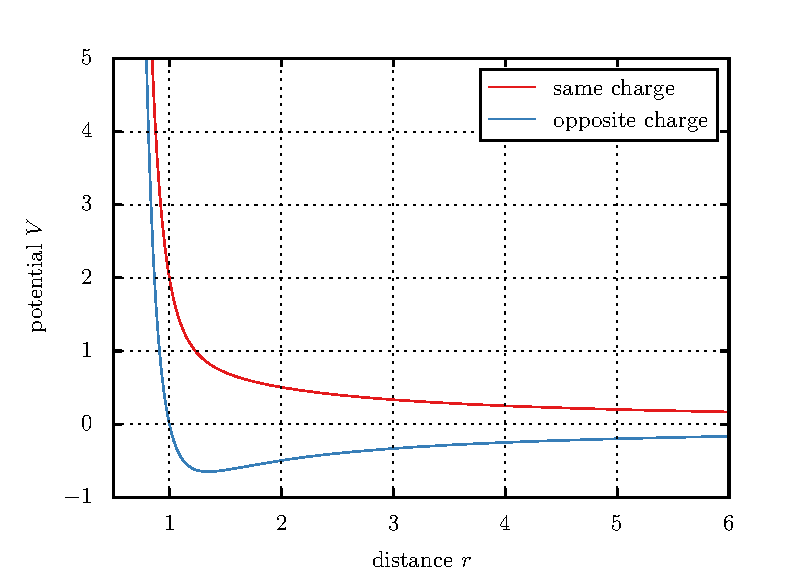
\includegraphics{./figures/potential_coulomb.pdf}
	\caption{Coulomb potential}
\end{figure}

\begin{figure}
	\centering
	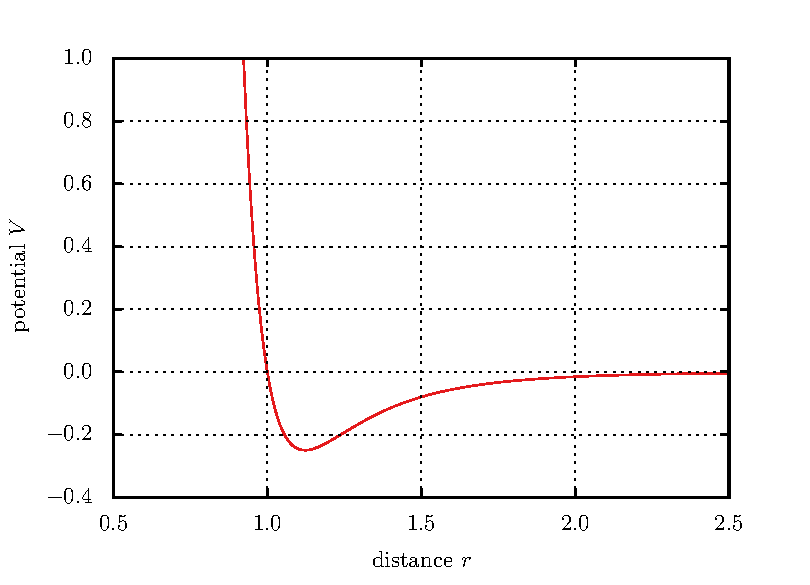
\includegraphics{./figures/potential_lennard_jones.pdf}
	\caption{Lennard-Jones potential}
\end{figure}

\begin{itemize}
	\item Coulomb with hard core
	\item Lennard-Jones
\end{itemize}

\subsection{Analysis of the Temperature Dependence} \label{sec:Temp_Dep}
To analyse the temperature dependence one can observe the average pair distance.
For the calculation of the average pair distance the formula
\begin{equation}
\frac{2}{N \cdot (N - 1)} \sum_{i<j} |\vec{r}_i - \vec{r}_j |
\end{equation}
is used.
$N$ is the number of particles (in the simulation is $N=40$) and $\vec{r}_i$, $\vec{r}_j$ are the positions of the $i$-th and $j$-th particle.
The calculation of the average pair distance is only done every \remark{k-th} step in order to save some computation time\footnote{A comparison between the calculation at every step and at every \remark{k-th} step was done.
The results do not differ.}.
The results of the average pair distance calculation was summed up and at the end of the simulation and than divided by the number of average pair distance calculations (to obtain the mean value of the average pair distance).
In order to estimate the uncertainty of the mean value of the average pair distance one simulates many times and analyses the distribution of the calculated values.
If one plots the mean value of the average pair distance against the temperature one can study the temperature dependence of the system.

\subsubsection{Two-dimensional case with Coulomb potential}
You can see in figure \ref{Fig:Temp_dep_Cou2D} the behaviour for the two-dimensional case with a Coulomb potential.
The red line is the mean value, the red area is the 1$\sigma$-range and in the grey area lie \SI{90}{\percent} of the calculated values.
About 24000 simulations where each simulation consists of one million steps were done to obtain this diagram.
Since it is useful to plot the \remark{$x$}-axis logarithmically it makes sense to make the step-size for $\beta$ exponentially.
The starting point for $\beta$ is 1 and the next $\beta$ is always \SI{4}{\percent} larger than the one before.
As an ending point a value of $\beta=500$ is reasonable.
Therefore there are 159 different values for $\beta$ in this diagram.

\begin{figure}[!h]
	\centering
	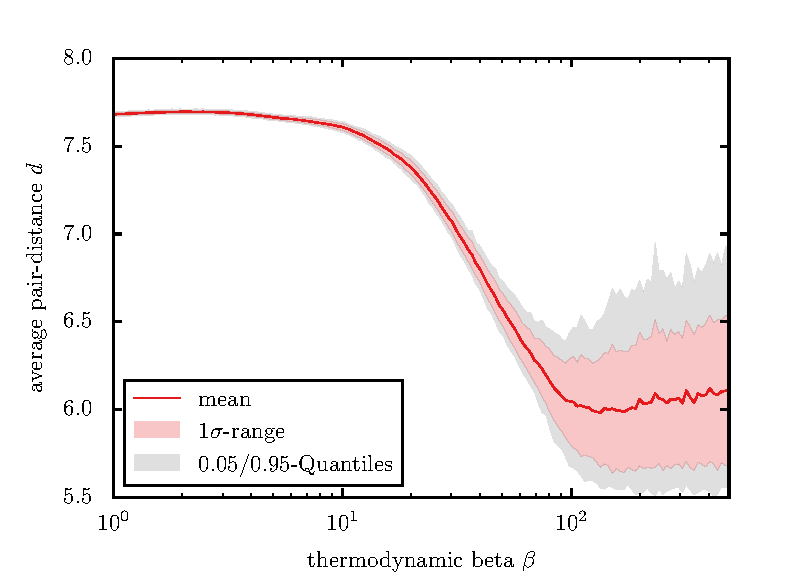
\includegraphics{./figures/temp_dep_coulomb2d.pdf}
	\caption{Temperature dependence 2d case}
	\label{Fig:Temp_dep_Cou2D}
\end{figure}

The diagram can be split into three parts.
In the following paragraphs those three parts will be analysed.
For a better understanding one can take a look at the figures in chapter \ref{sec:Visualisation}.

\begin{itemize}
\item{\remark{Gaseous state} ($\beta \lesssim 10)$:}

The average pair distance is high for high temperatures (high temperatures are equivalent to low $\beta$).
One expects this behaviour since for high temperatures the system is in a gaseous state.
The distance between two particles is maximal in a gaseous system.
Also one can clearly see that the uncertainty is very small.
The interpretation of this small uncertainty is that the gas uses the whole volume of the box.
Therefore one averages always over the whole box which leads to a small uncertainty.

\item{\remark{Liquid State} ($10 \lesssim \beta \lesssim 100)$:}

For higher $\beta$ the average pair distance drops.
This happens at $\beta \approx 10$.
From this point on the system is in a liquid-like state.
The particles are getting closer together which one can interpret as the formation of particle chains.
This can be understand if one takes a closer look to equation \ref{Eq:Prob_New_State}.
The probability that a new proposed state is accepted depends on $\beta$.
With higher $\beta$ the factor $\alpha$ gets small if $E_\mathrm{prop.} > E_\mathrm{cur.}$ and it is not likely that a $\mathcal{U}(0, 1)$-distributed random variable is smaller than $\alpha$.
But if the other case happens ($E_\mathrm{prop.} < E_\mathrm{cur.}$) the factor $\alpha$ is always larger than 1 and therefore the proposed state will be accepted.

\item{\remark{Solid State} ($100 \lesssim \beta$):}

The average pair distance for high $\beta$ is almost constant.
One can interpret this as a solid state.
If the particles form a solid state the particles can not come closer for smaller temperatures since the potential has a minimum (as discussed in chapter \ref{sec:Potentials}). \remark{Hier noch mehr?!}
The reason that the particles form a solid state with a small distance is comparable to the argumentation that was used to explain the liquid state.
In the case of very high $\beta$ the factor $\alpha$ is very small even if the proposed energy $E_\mathrm{prop.}$ is just slightly larger than the current energy $E_\mathrm{cur.}$.
Therefore it is very unlikely that a state forms where the proposed energy is higher than the current energy.

In the diagram one can also observe a huge uncertainty for high $\beta$.
The explanation for this behaviour is the formation of crystallographic defects.
If a crystal is in a state where it is not possible to form a regular grid (maybe due to a missing charge, a rotation of some structures \dots) the crystal will have a large expansion.
Since the formation of crystallographic defects is random it leads to an uncertainty in the average pair distance.
\end{itemize}

\subsubsection{Two-dimensional case with Lennard-Jones potential}
If the Coulomb potential is exchanged with a Lennard-Jones potential \remark{Gleichung referenzieren} the dependence on $\beta$ changes.
The plot in figure \ref{Fig:Temp_dep_LJ2D} is basically the same as the plot in figure \ref{Fig:Temp_dep_Cou2D} but the potential is now a Lennard-Jones potential.
One can clearly see that the behaviour for low values of $\beta$ is the same as for the Coulomb potential.
For higher values of $\beta$ the average pair distance drops.
After the average pair distance reaches its smallest value it begins to rise again.
The Lennard-Jones potential has only a short range.
This short range is responsible for this behaviour since some crystal-like state can form but once it has formed it stays on the same place and can not connect with other crystals which are formed somewhere else.
Some pictures of the final states can be found in chapter \ref{sec:Visualisation}.

\begin{figure}
	\centering
	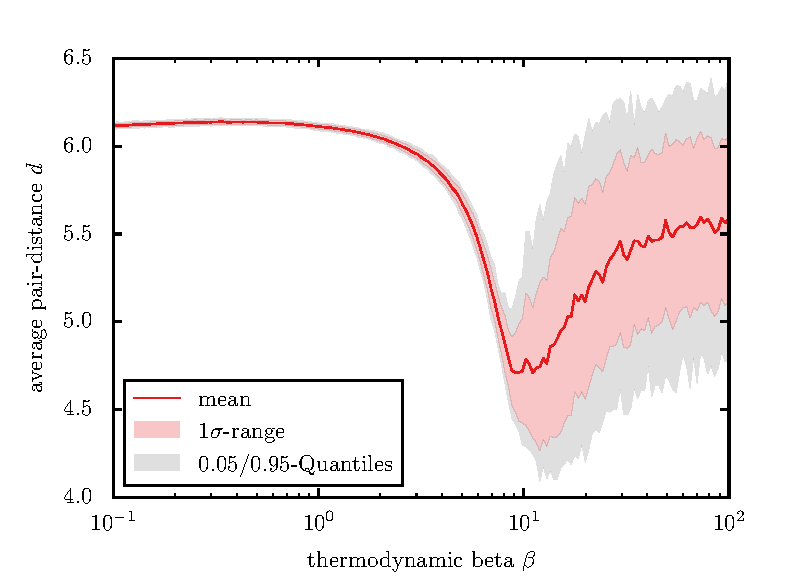
\includegraphics{./figures/temp_dep_lennard_jones2d.pdf}
	\caption{Temperature dependence 3d case \remark{Lennard Jones 2D?}}
	\label{Fig:Temp_dep_LJ2D}
\end{figure}

\subsubsection{Three-dimensional case with Coulomb potential}
\begin{figure}
	\centering
	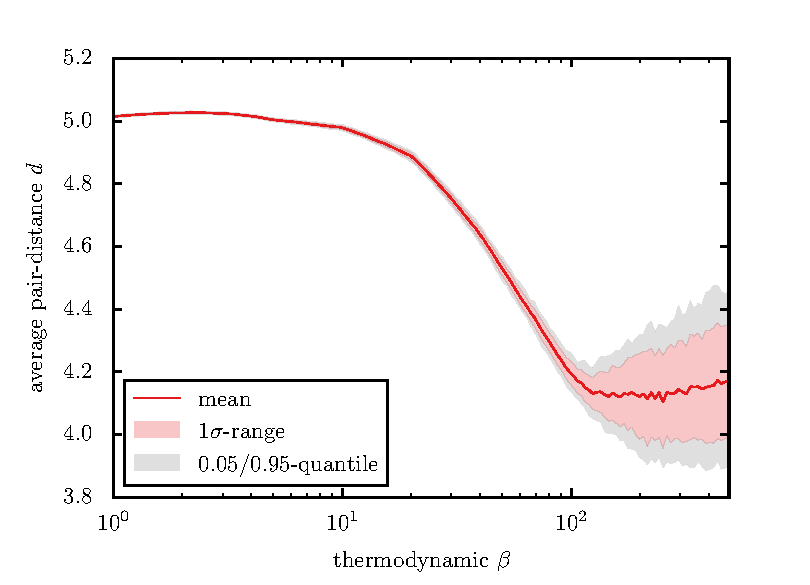
\includegraphics{./figures/temp_dep_coulomb3d.pdf}
	\caption{Temperature dependence 3d case}
\end{figure}



\subsection{Visualization} \label{sec:Visualisation}
In this section a few examples of the resulting final states are shown.
For each picture a simulation with one million steps was performed.
The position of the particles in the last step were saved and a python script (using the library \texttt{matplotlib}) created an image.

\begin{figure}[!h]
\centering
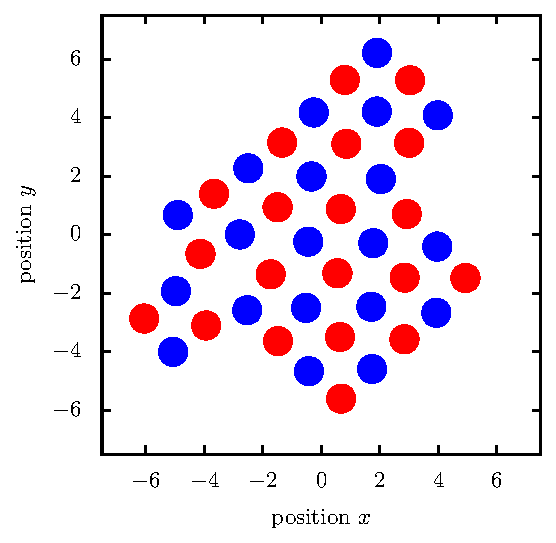
\includegraphics[scale=1]{figures/Kristall_3_beta_500.pdf}
\caption{Final state for $\beta = 500$. 
One can clearly see that this low temperature leads to a crystal (solid state). 
The average pair distance is very small and regularly.
Only a few crystallographic defects appear.}
\end{figure}

\begin{figure}[!h]
\centering
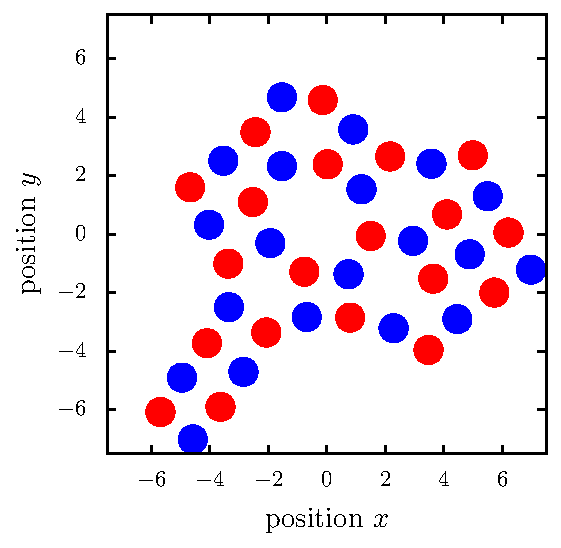
\includegraphics[scale=1]{figures/Kristall_4_beta_500.pdf}
\caption{Final state again for $\beta = 500$. 
The average pair distance is slightly larger and the lattice is not regularly.
A lot of crystallographic defects appear.
This is the reason for the large uncertainty which was discussed in section \ref{sec:Temp_Dep}.}
\end{figure}

\begin{figure}[!h]
\centering
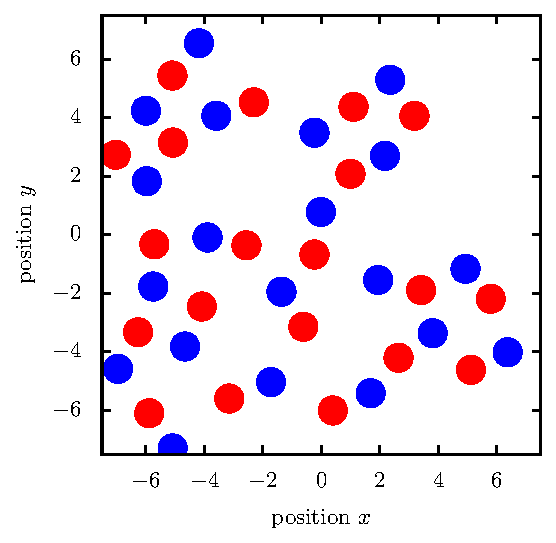
\includegraphics[scale=1]{figures/Fluid_1_beta_40.pdf}
\caption{Final state for $\beta = 40$.
A higher temperature leads to an amorphous state (fluid).
The average pair distance is larger and the lattice is completely gone.
One can observe some strings and some particles which form a pair.}
\end{figure}


\begin{figure}[!h]
\centering
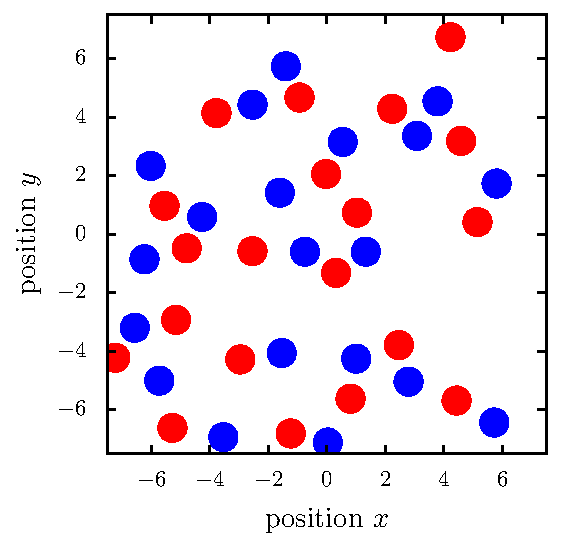
\includegraphics[scale=1]{figures/Gas_1_beta_10.pdf}
\caption{Final state for $\beta = 10$.
An even higher temperature leads to an gaseous state.
The average pair distance is at its maximum since the particles are more or less randomly distributed over the whole box.
Additionally the strings which were observed at the amorphous state are now shorter.
Often two particles form a pair.}
\end{figure}


\begin{figure}[!h]
\centering
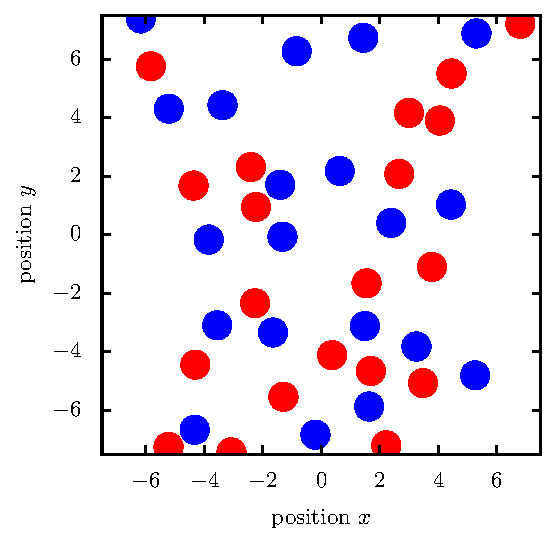
\includegraphics[scale=1]{figures/Plasma_1_beta_2.pdf}
\caption{Final state for $\beta = 2$.
At very high temperatures the particles are in a plasma-like state since the particles rarely form pairs.
Sometimes two particles with the same charge are very close together.}
\end{figure}
\remark{3D Visualization?}


\section{Further Analysis} \label{sec:Further_Analysis}



\FloatBarrier
% BIBLIOGRAPHY
\vspace{\fill}
\begin{thebibliography}{9}
\bibitem{schwabl}
	F. Schwabl,
	\emph{Statistische Mechanik},
	Springer, Berlin, 3rd edition 2006.
\end{thebibliography}

\begin{appendix}
	\newpage
	\section{Source code}
	The full source code can be found on \url{https://github.com/chrisieh/piap} (a \texttt{C++14} compliant compiler is needed).
	\subsection{CanonicalEnsemble{.}h} \label{sec:canonical_ensemble_source}
	\lstinputlisting[language=C++]{../code/src/CanonicalEnsemble.h}
\end{appendix}

\end{document}